% Author: Izaak Neutelings (July 2018)
\documentclass[border=3pt,tikz]{standalone}
\usepackage{tikz}
\usepackage{physics}
\tikzset{>=latex} % for LaTeX arrow head
\usetikzlibrary{angles,quotes} % for pic (angle labels)
\usepackage{xcolor}
\colorlet{pinkskin}{pink!25}
\colorlet{brownskin}{pink!5!brown!45}
\colorlet{myred}{red!90!black}
\colorlet{myblue}{blue!90!black}
\colorlet{mypurple}{blue!50!red!80!black!80}
\colorlet{Bcol}{violet!90}
\colorlet{BFcol}{red!60!black}
\colorlet{veccol}{green!45!black}
\colorlet{Icol}{blue!70!black}
\colorlet{mucol}{red!90!black}
\tikzstyle{BField}=[->,line width=2,Bcol]
\tikzstyle{current}=[->,Icol] %thick,
\tikzstyle{force}=[->,line width=2,BFcol]
\tikzstyle{vector}=[->,line width=2,veccol]
\tikzstyle{thick vector}=[->,line width=2,veccol]
\tikzstyle{mu vector}=[->,line width=2,mucol]
\tikzstyle{velocity}=[->,line width=2,veccol]
\tikzstyle{charge+}=[very thin,draw=black,top color=red!50,bottom color=red!90!black,shading angle=20,circle,inner sep=0.5]


\begin{document}
\Large


% RIGHT HAND RULE F = qvxB (brown)
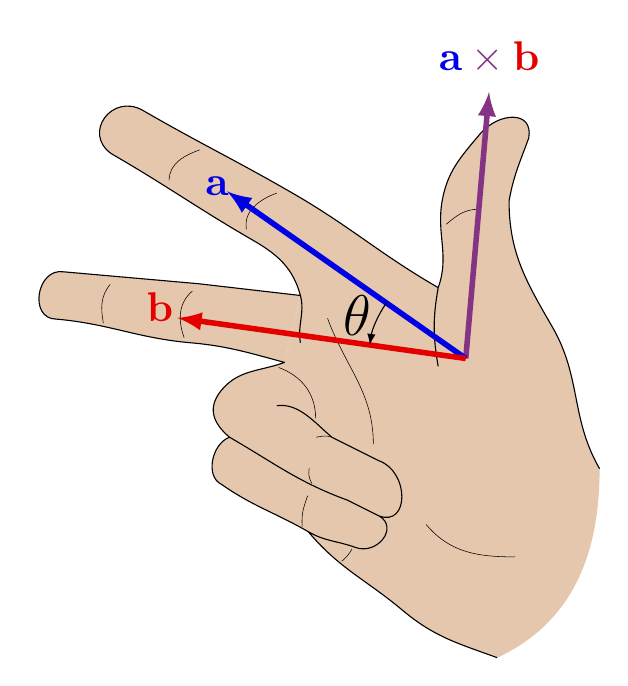
\begin{tikzpicture}
  \coordinate (O) at (1.2,0.3); % ORIGIN
  \coordinate (WT) at ( 2.9,-1.1); % WRIST TOP
  \coordinate (T1) at ( 2.3, 0.7); % THUMB
  \coordinate (T2) at ( 1.75, 2.3);
  \coordinate (T3) at ( 2.0, 3.1);
  \coordinate (T4) at (1.38, 3.15);
  \coordinate (T5) at ( 0.9, 2.3);
  \coordinate (T6) at ( 0.85, 1.2);
  \coordinate (T7) at ( 0.85, 0.2);
  \coordinate (I1) at (-1.0, 2.4); % INDEX
  \coordinate (I2) at (-2.9, 3.45);
  \coordinate (I3) at (-3.3, 2.9);
  \coordinate (I4) at (-1.5, 1.8);
  \coordinate (I5) at (-0.9, 1.1);
  \coordinate (I6) at (-0.9, 0.5);
  \coordinate (M1) at (-2.2, 1.25); % MIDDLE
  \coordinate (M2) at (-3.9, 1.4);
  \coordinate (M3) at (-4.0, 0.8);
  \coordinate (M4) at (-2.3, 0.5);
  \coordinate (M5) at (-1.1, 0.25);
  \coordinate (R1) at (-1.9,-0.1); % RING
  \coordinate (R2) at (-1.8,-0.7);
  \coordinate (R3) at (-0.3,-1.5);
  \coordinate (R4) at ( 0.1,-1.7);
  \coordinate (R5) at ( 0.1,-1.0);
  \coordinate (R6) at (-0.5,-0.7);
  \coordinate (R7) at (-1.2,-0.3);
  \coordinate (P1) at (-1.9,-1.3); % PINKY
  \coordinate (P2) at (-0.8,-1.9);
  \coordinate (P3) at (-0.2,-2.1);
  \coordinate (P4) at (-0.05,-1.65);
  \coordinate (W1) at ( 0.4,-2.9); % WRIST BOTTOM
  \coordinate (W2) at ( 1.6,-3.5);
  
  % HAND
  \fill[brownskin]
    (WT) -- (T6) -- (I5) -- (M5) -- (R2) -- (P2) -- (W2) to[out=25,in=-90] cycle;
  \draw[fill=brownskin]
    (WT) to[out=120,in=-60] % THUMB
    (T1) to[out=120,in=-90]
    (T2) to[out=80,in=-110]
    (T3) to[out=80,in=50,looseness=1.5] % tip
    (T4) to[out=-130,in=80]
    (T5) to[out=-100,in=70]
    (T6) to[out=-100,in=100]
    (T7)
    (T6) to[out=150,in=-30] % INDEX
    (I1) to[out=150,in=-30]
    (I2) to[out=150,in=145,looseness=1.7] % tip
    (I3) to[out=-30,in=150]
    (I4) to[out=-30,in=105]
    (I5) to[out=-75,in=100]
    (I6)
    (I5) -- % MIDDLE
    (M1) --
    (M2) to[out=170,in=180,looseness=1.5] % tip
    (M3) to[out=-5,in=175]
    (M4) to[out=-5,in=165] % bottom knuckle
    (M5)
    (M5) to[out=-160,in=50] % RING
    (R1) to[out=-130,in=140,looseness=1.2]
    (R2) to[out=-30,in=160]
    (R3) --
    (R4) to[out=-20,in=-20,looseness=1.5] % tip
    (R5) --
    (R6) to[out=140,in=8,looseness=0.9]
    (R7)
    (R2) to[out=-160,in=155] % PINKY
    (P1) to[out=-35,in=150]
    (P2) to[out=-30,in=160]
    (P3) to[out=-20,in=-30,looseness=1.5] % tip
    %(P4) --
    (R4)
    (P2) to[out=-50,in=140] % WRIST
    (W1) to[out=-40,in=160]
    (W2);
  
  % FOLDS
  \draw[very thin] (T5)++(-80:0.3) to[out=40,in=180]++ (25:0.45);
  \draw[very thin] (I1)++(180:0.2) to[out=-160,in=100]++ (-130:0.6);
  \draw[very thin] (I1)++(155:1.3) to[out=-160,in=90]++ (-135:0.55);
  \draw[very thin] (M4)++(140:0.1) to[out=110,in=-140]++ (80:0.6);
  \draw[very thin] (M3)++(-5:0.6) to[out=100,in=-130]++ (80:0.5);
  \draw[very thin] (M5)++(-140:0.1) to[out=-20,in=90]++ (-54:0.8); % RING
  \draw[very thin] (R6) to[out=160,in=10]++ (180:0.2);
  \draw[very thin] (R3)++(155:0.5) to[out=120,in=-100]++ (100:0.2);
  \draw[very thin] (P2)++(140:0.1) to[out=95,in=-110]++ (80:0.4);
  %\draw[very thin] (P1)++( 10:0.04) to[out=95,in=-130]++ (70:0.4);
  \draw[very thin] (I5)++(-40:0.45) to[out=-70,in=90]++ (-70:1.7);    % PALM
  \draw[very thin] (P3)++(-155:0.05) to[out=-120,in=40]++ (-130:0.2); % PALM
  \draw[very thin] (W2)++(80:1.3) to[out=-180,in=-50]++ (160:1.2); % PALM
  
  % VECTORS
  \draw[thick vector,mypurple]
    (O) --++ (85:3.4)
    node[above,scale=1.5] {${\color{myblue}\vb{a}} \times {\color{myred}\vb{b}}$};
  \draw[thick vector,myblue]
    (O) --++ (145:3.7) coordinate (A)
    node[above=2,left=-7,scale=1.5] {$\vb{a}$};
  \draw[thick vector,myred]
    (O) --++ (172:3.7) coordinate (B)
    node[above=4,left=-5,scale=1.5] {$\vb{b}$};
  \draw pic[->,"\huge$\theta$",draw=black,angle radius=35,angle eccentricity=1.2] {angle = A--O--B};
  
  % HELP LINES
%  \foreach \i in {0,...,4}{
%    \draw[very thin,red!10] (-4.5, \i) -- (4, \i);
%    \draw[very thin,red!10] (-4.5,-\i) -- (4,-\i);
%    \draw[very thin,red!10] (\i,-4) -- (\i,4);
%    \draw[very thin,red!10] (-\i,-4) -- (-\i,4);
%  }
%  \node[blue,scale=0.4] at (T1) {T1};
%  \node[blue,scale=0.4] at (T2) {T2};
%  \node[blue,scale=0.4] at (T3) {T3};
%  \node[blue,scale=0.4] at (T4) {T4};
%  \node[blue,scale=0.4] at (T5) {T5};
%  \node[blue,scale=0.4] at (T6) {T6};
%  \node[blue,scale=0.4] at (T7) {T7};
%  \node[blue,scale=0.4] at (I1) {I1};
%  \node[blue,scale=0.4] at (I2) {I2};
%  \node[blue,scale=0.4] at (I3) {I3};
%  \node[blue,scale=0.4] at (I4) {I4};
%  \node[blue,scale=0.4] at (I5) {I5};
%  \node[blue,scale=0.4] at (M1) {M1};
%  \node[blue,scale=0.4] at (M2) {M2};
%  \node[blue,scale=0.4] at (M3) {M3};
%  \node[blue,scale=0.4] at (M4) {M4};
%  \node[blue,scale=0.4] at (M5) {M5};
%  \node[blue,scale=0.4] at (R1) {R1};
%  \node[blue,scale=0.4] at (R2) {R2};
%  \node[blue,scale=0.4] at (R3) {R3};
%  \node[blue,scale=0.4] at (R4) {R4};
%  \node[blue,scale=0.4] at (R5) {R5};
%  \node[blue,scale=0.4] at (R6) {R6};
%  \node[blue,scale=0.4] at (R7) {R7};
%  \node[blue,scale=0.4] at (P1) {P1};
%  \node[blue,scale=0.4] at (P2) {P2};
%  \node[blue,scale=0.4] at (P3) {P3};
%  %\node[blue,scale=0.4] at (P4) {P4};
%  \node[blue,scale=0.4] at (W1) {W1};
%  \node[blue,scale=0.4] at (W2) {W2};
  
\end{tikzpicture}


% RIGHT HAND RULE xyz
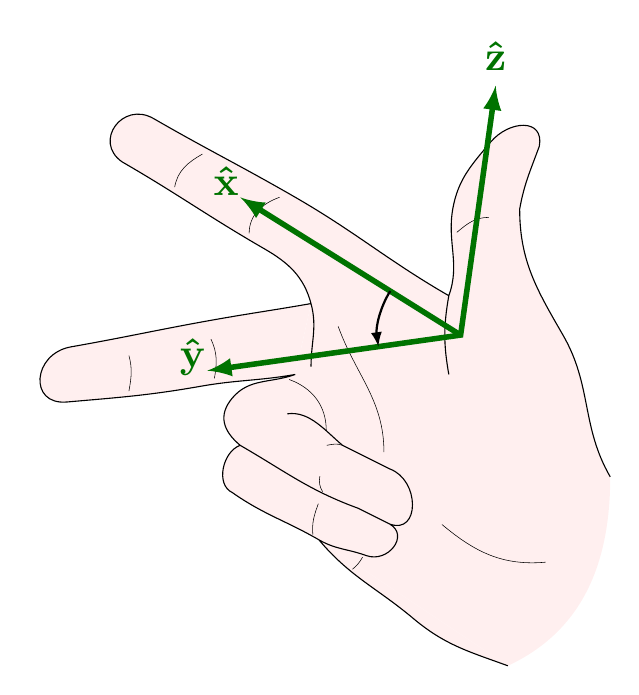
\begin{tikzpicture}
  \coordinate (O) at (1.0,0.7); % ORIGIN
  \coordinate (WT) at ( 2.9,-1.1); % WRIST TOP
  \coordinate (T1) at ( 2.3, 0.7); % THUMB
  \coordinate (T2) at ( 1.75, 2.3);
  \coordinate (T3) at ( 2.0, 3.1);
  \coordinate (T4) at (1.38, 3.15);
  \coordinate (T5) at ( 0.9, 2.3);
  \coordinate (T6) at ( 0.85, 1.2);
  \coordinate (T7) at ( 0.85, 0.2);
  \coordinate (I1) at (-1.1, 2.45); % INDEX
  \coordinate (I2) at (-2.9, 3.45);
  \coordinate (I3) at (-3.3, 2.9);
  \coordinate (I4) at (-1.5, 1.8);
  \coordinate (I5) at (-0.9, 1.1);
  \coordinate (I6) at (-0.9, 0.3);
  \coordinate (M1) at (-2.1, 0.9); % MIDDLE
  \coordinate (M2) at (-3.95,0.55);
  \coordinate (M3) at (-4.0,-0.15);
  \coordinate (M4) at (-2.3, 0.05);
  \coordinate (M5) at (-1.1, 0.20);
  \coordinate (R1) at (-1.9,-0.1); % RING
  \coordinate (R2) at (-1.8,-0.7);
  \coordinate (R3) at (-0.3,-1.5);
  \coordinate (R4) at ( 0.1,-1.7);
  \coordinate (R5) at ( 0.1,-1.0);
  \coordinate (R6) at (-0.5,-0.7);
  \coordinate (R7) at (-1.2,-0.3);
  \coordinate (P1) at (-1.9,-1.3); % PINKY
  \coordinate (P2) at (-0.8,-1.9);
  \coordinate (P3) at (-0.2,-2.1);
  \coordinate (P4) at (-0.05,-1.65);
  \coordinate (W1) at ( 0.4,-2.9); % WRIST BOTTOM
  \coordinate (W2) at ( 1.6,-3.5);
  
  % HAND
  \fill[pinkskin]
    (WT) -- (T6) -- (I5) -- (M5) -- (R2) -- (P2) -- (W2) to[out=25,in=-90] cycle;
  \draw[fill=pinkskin]
    (WT) to[out=120,in=-60] % THUMB
    (T1) to[out=120,in=-90]
    (T2) to[out=80,in=-110]
    (T3) to[out=80,in=50,looseness=1.5] % tip
    (T4) to[out=-130,in=80]
    (T5) to[out=-100,in=70]
    (T6) to[out=-100,in=100]
    (T7)
    (T6) to[out=150,in=-30] % INDEX
    (I1) to[out=150,in=-30]
    (I2) to[out=150,in=145,looseness=1.7] % tip
    (I3) to[out=-30,in=150]
    (I4) to[out=-30,in=105]
    (I5) to[out=-75,in=90]
    (I6)
    (I5) to[out=-170,in=10] % MIDDLE
    (M1) to[out=-170,in=10]
    (M2) to[out=-170,in=-175,looseness=1.8] % tip
    (M3) to[out=5,in=-170]
    (M4) to[out=10,in=-170] % bottom knuckle
    (M5)
    (M5) to[out=-160,in=50] % RING
    (R1) to[out=-130,in=140,looseness=1.2]
    (R2) to[out=-30,in=160]
    (R3) --
    (R4) to[out=-20,in=-20,looseness=1.5] % tip
    (R5) --
    (R6) to[out=140,in=8,looseness=0.9]
    (R7)
    (R2) to[out=-160,in=155] % PINKY
    (P1) to[out=-35,in=150]
    (P2) to[out=-30,in=160]
    (P3) to[out=-20,in=-30,looseness=1.5] % tip
    %(P4) --
    (R4)
    (P2) to[out=-50,in=140] % WRIST
    (W1) to[out=-40,in=160]
    (W2);
  
  % FOLDS
  \draw[very thin] (T5)++(-80:0.3) to[out=40,in=180]++ (25:0.45); % THUMB
  \draw[very thin] (I1)++(180:0.2) to[out=-160,in=90]++ (-130:0.6); % INDEX
  \draw[very thin] (I1)++(155:1.3) to[out=-150,in=80]++ (-130:0.55);
  \draw[very thin] (M4)++(30:0.2) to[out=80,in=-65]++ (95:0.5); % MIDDLE FINGER
  \draw[very thin] (M3)++(10:0.8) to[out=80,in=-75]++ (90:0.45);
  \draw[very thin] (M5)++(-140:0.1) to[out=-20,in=90]++ (-54:0.8); % RING
  \draw[very thin] (R6) to[out=160,in=10]++ (180:0.2);
  \draw[very thin] (R3)++(155:0.5) to[out=120,in=-100]++ (100:0.2);
  \draw[very thin] (P2)++(140:0.1) to[out=95,in=-110]++ (80:0.4); % PINKY
  %\draw[very thin] (P1)++( 10:0.04) to[out=95,in=-130]++ (70:0.4);
  \draw[very thin] (I5)++(-40:0.45) to[out=-70,in=90]++ (-70:1.7);    % PALM
  \draw[very thin] (P3)++(-155:0.05) to[out=-120,in=40]++ (-130:0.2); % PALM
  \draw[very thin] (W2)++(70:1.4) to[out=-175,in=-40]++ (160:1.4); % PALM
  
  % VECTORS
  \def\R{0.32}
  \draw[thick vector]
    (O) --++ (148:3.3) coordinate (X) node[above=6,left=-6,scale=1.5] {$\vu{x}$};
  \draw[thick vector,<->]
    (O) ++ (-172:3.25) coordinate (Y) node[above=5,left=-6,scale=1.5] {$\vu{y}$} --
    (O) --++ (82:3.2) node[above=-1,scale=1.5] {$\vu{z}$};
  \draw pic[->,draw=black,thick,angle radius=30,angle eccentricity=1.2] {angle = X--O--Y};
  
\end{tikzpicture}


% RIGHT HAND RULE: F = qvxB
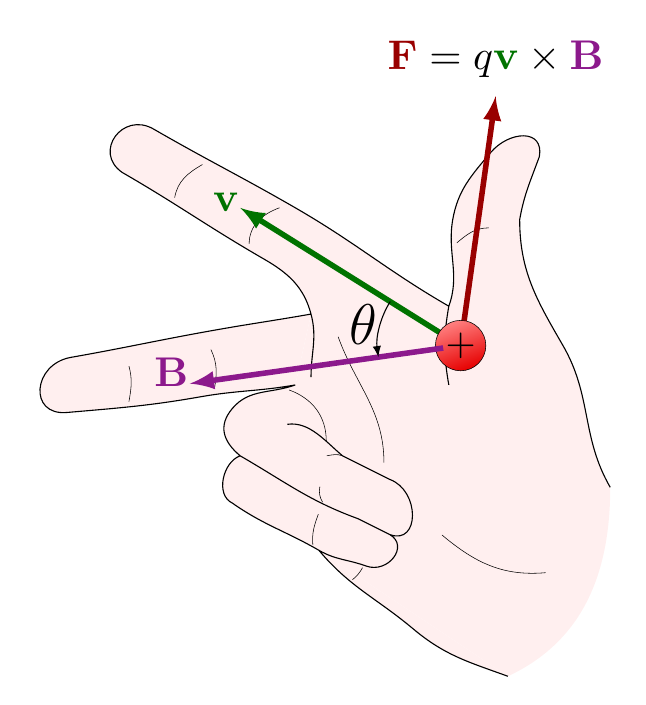
\begin{tikzpicture}
  \coordinate (O) at (1.0,0.7); % ORIGIN
  \coordinate (WT) at ( 2.9,-1.1); % WRIST TOP
  \coordinate (T1) at ( 2.3, 0.7); % THUMB
  \coordinate (T2) at ( 1.75, 2.3);
  \coordinate (T3) at ( 2.0, 3.1);
  \coordinate (T4) at (1.38, 3.15);
  \coordinate (T5) at ( 0.9, 2.3);
  \coordinate (T6) at ( 0.85, 1.2);
  \coordinate (T7) at ( 0.85, 0.2);
  \coordinate (I1) at (-1.1, 2.45); % INDEX
  \coordinate (I2) at (-2.9, 3.45);
  \coordinate (I3) at (-3.3, 2.9);
  \coordinate (I4) at (-1.5, 1.8);
  \coordinate (I5) at (-0.9, 1.1);
  \coordinate (I6) at (-0.9, 0.3);
  \coordinate (M1) at (-2.1, 0.9); % MIDDLE
  \coordinate (M2) at (-3.95,0.55);
  \coordinate (M3) at (-4.0,-0.15);
  \coordinate (M4) at (-2.3, 0.05);
  \coordinate (M5) at (-1.1, 0.20);
  \coordinate (R1) at (-1.9,-0.1); % RING
  \coordinate (R2) at (-1.8,-0.7);
  \coordinate (R3) at (-0.3,-1.5);
  \coordinate (R4) at ( 0.1,-1.7);
  \coordinate (R5) at ( 0.1,-1.0);
  \coordinate (R6) at (-0.5,-0.7);
  \coordinate (R7) at (-1.2,-0.3);
  \coordinate (P1) at (-1.9,-1.3); % PINKY
  \coordinate (P2) at (-0.8,-1.9);
  \coordinate (P3) at (-0.2,-2.1);
  \coordinate (P4) at (-0.05,-1.65);
  \coordinate (W1) at ( 0.4,-2.9); % WRIST BOTTOM
  \coordinate (W2) at ( 1.6,-3.5);
  
  % HAND
  \fill[pinkskin]
    (WT) -- (T6) -- (I5) -- (M5) -- (R2) -- (P2) -- (W2) to[out=25,in=-90] cycle;
  \draw[fill=pinkskin]
    (WT) to[out=120,in=-60] % THUMB
    (T1) to[out=120,in=-90]
    (T2) to[out=80,in=-110]
    (T3) to[out=80,in=50,looseness=1.5] % tip
    (T4) to[out=-130,in=80]
    (T5) to[out=-100,in=70]
    (T6) to[out=-100,in=100]
    (T7)
    (T6) to[out=150,in=-30] % INDEX
    (I1) to[out=150,in=-30]
    (I2) to[out=150,in=145,looseness=1.7] % tip
    (I3) to[out=-30,in=150]
    (I4) to[out=-30,in=105]
    (I5) to[out=-75,in=90]
    (I6)
    (I5) to[out=-170,in=10] % MIDDLE
    (M1) to[out=-170,in=10]
    (M2) to[out=-170,in=-175,looseness=1.8] % tip
    (M3) to[out=5,in=-170]
    (M4) to[out=10,in=-170] % bottom knuckle
    (M5)
    (M5) to[out=-160,in=50] % RING
    (R1) to[out=-130,in=140,looseness=1.2]
    (R2) to[out=-30,in=160]
    (R3) --
    (R4) to[out=-20,in=-20,looseness=1.5] % tip
    (R5) --
    (R6) to[out=140,in=8,looseness=0.9]
    (R7)
    (R2) to[out=-160,in=155] % PINKY
    (P1) to[out=-35,in=150]
    (P2) to[out=-30,in=160]
    (P3) to[out=-20,in=-30,looseness=1.5] % tip
    %(P4) --
    (R4)
    (P2) to[out=-50,in=140] % WRIST
    (W1) to[out=-40,in=160]
    (W2);
  
  % FOLDS
  \draw[very thin] (T5)++(-80:0.3) to[out=40,in=180]++ (25:0.45); % THUMB
  \draw[very thin] (I1)++(180:0.2) to[out=-160,in=90]++ (-130:0.6); % INDEX
  \draw[very thin] (I1)++(155:1.3) to[out=-150,in=80]++ (-130:0.55);
  \draw[very thin] (M4)++(30:0.2) to[out=80,in=-65]++ (95:0.5); % MIDDLE FINGER
  \draw[very thin] (M3)++(10:0.8) to[out=80,in=-75]++ (90:0.45);
  \draw[very thin] (M5)++(-140:0.1) to[out=-20,in=90]++ (-54:0.8); % RING
  \draw[very thin] (R6) to[out=160,in=10]++ (180:0.2);
  \draw[very thin] (R3)++(155:0.5) to[out=120,in=-100]++ (100:0.2);
  \draw[very thin] (P2)++(140:0.1) to[out=95,in=-110]++ (80:0.4); % PINKY
  %\draw[very thin] (P1)++( 10:0.04) to[out=95,in=-130]++ (70:0.4);
  \draw[very thin] (I5)++(-40:0.45) to[out=-70,in=90]++ (-70:1.7);    % PALM
  \draw[very thin] (P3)++(-155:0.05) to[out=-120,in=40]++ (-130:0.2); % PALM
  \draw[very thin] (W2)++(70:1.4) to[out=-175,in=-40]++ (160:1.4); % PALM
  
  % VECTORS
  \def\R{0.32}
  \draw[force]
    (O) --++ (82:3.2)
    node[above,scale=1.5] {$\vb{F} \color{black} = q {\color{veccol}\vb{v}} \times {\color{Bcol}\vb{B}}$};
  \draw[velocity]
    (O) --++ (148:3.3) coordinate (V)
    node[above=2,left=-6,scale=1.5] {$\vb{v}$};
  \draw[charge+] (O) circle (\R) node[scale=1.4] {$+$};
  \draw[BField]
    (O)++(-172:0.7*\R) --++ (-172:3.25) coordinate (B)
    node[above=4,left=-6,scale=1.5] {$\vb{B}$};
  \draw pic[->,"\huge$\theta$",draw=black,angle radius=30,angle eccentricity=1.2] {angle = V--O--B};
  
%  % HELP LINES
%  \foreach \i in {0,...,4}{
%    \draw[very thin,red!10] (-4.5, \i) -- (4, \i);
%    \draw[very thin,red!10] (-4.5,-\i) -- (4,-\i);
%    \draw[very thin,red!10] (\i,-4) -- (\i,4);
%    \draw[very thin,red!10] (-\i,-4) -- (-\i,4);
%  }
%  \node[blue,scale=0.4] at (T1) {T1};
%  \node[blue,scale=0.4] at (T2) {T2};
%  \node[blue,scale=0.4] at (T3) {T3};
%  \node[blue,scale=0.4] at (T4) {T4};
%  \node[blue,scale=0.4] at (T5) {T5};
%  \node[blue,scale=0.4] at (T6) {T6};
%  \node[blue,scale=0.4] at (T7) {T7};
%  \node[blue,scale=0.4] at (I1) {I1};
%  \node[blue,scale=0.4] at (I2) {I2};
%  \node[blue,scale=0.4] at (I3) {I3};
%  \node[blue,scale=0.4] at (I4) {I4};
%  \node[blue,scale=0.4] at (I5) {I5};
%  \node[blue,scale=0.4] at (M1) {M1};
%  \node[blue,scale=0.4] at (M2) {M2};
%  \node[blue,scale=0.4] at (M3) {M3};
%  \node[blue,scale=0.4] at (M4) {M4};
%  \node[blue,scale=0.4] at (M5) {M5};
%  \node[blue,scale=0.4] at (R1) {R1};
%  \node[blue,scale=0.4] at (R2) {R2};
%  \node[blue,scale=0.4] at (R3) {R3};
%  \node[blue,scale=0.4] at (R4) {R4};
%  \node[blue,scale=0.4] at (R5) {R5};
%  \node[blue,scale=0.4] at (R6) {R6};
%  \node[blue,scale=0.4] at (R7) {R7};
%  \node[blue,scale=0.4] at (P1) {P1};
%  \node[blue,scale=0.4] at (P2) {P2};
%  \node[blue,scale=0.4] at (P3) {P3};
%  %\node[blue,scale=0.4] at (P4) {P4};
%  \node[blue,scale=0.4] at (W1) {W1};
%  \node[blue,scale=0.4] at (W2) {W2};
  
\end{tikzpicture}


% RIGHT HAND RULE F = qvxB (brown)
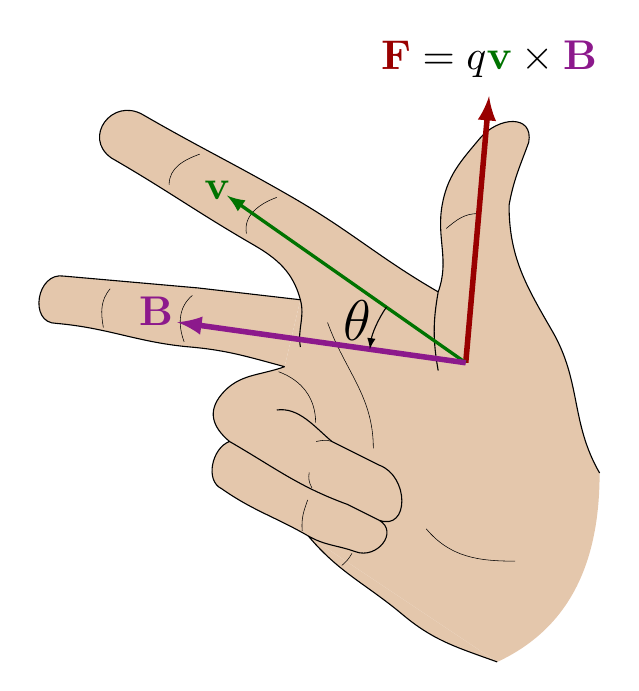
\begin{tikzpicture}
  \coordinate (O) at (1.2,0.3); % ORIGIN
  \coordinate (WT) at ( 2.9,-1.1); % WRIST TOP
  \coordinate (T1) at ( 2.3, 0.7); % THUMB
  \coordinate (T2) at ( 1.75, 2.3);
  \coordinate (T3) at ( 2.0, 3.1);
  \coordinate (T4) at (1.38, 3.15);
  \coordinate (T5) at ( 0.9, 2.3);
  \coordinate (T6) at ( 0.85, 1.2);
  \coordinate (T7) at ( 0.85, 0.2);
  \coordinate (I1) at (-1.0, 2.4); % INDEX
  \coordinate (I2) at (-2.9, 3.45);
  \coordinate (I3) at (-3.3, 2.9);
  \coordinate (I4) at (-1.5, 1.8);
  \coordinate (I5) at (-0.9, 1.1);
  \coordinate (I6) at (-0.9, 0.5);
  \coordinate (M1) at (-2.2, 1.25); % MIDDLE
  \coordinate (M2) at (-3.9, 1.4);
  \coordinate (M3) at (-4.0, 0.8);
  \coordinate (M4) at (-2.3, 0.5);
  \coordinate (M5) at (-1.1, 0.25);
  \coordinate (R1) at (-1.9,-0.1); % RING
  \coordinate (R2) at (-1.8,-0.7);
  \coordinate (R3) at (-0.3,-1.5);
  \coordinate (R4) at ( 0.1,-1.7);
  \coordinate (R5) at ( 0.1,-1.0);
  \coordinate (R6) at (-0.5,-0.7);
  \coordinate (R7) at (-1.2,-0.3);
  \coordinate (P1) at (-1.9,-1.3); % PINKY
  \coordinate (P2) at (-0.8,-1.9);
  \coordinate (P3) at (-0.2,-2.1);
  \coordinate (P4) at (-0.05,-1.65);
  \coordinate (W1) at ( 0.4,-2.9); % WRIST BOTTOM
  \coordinate (W2) at ( 1.6,-3.5);
  
  % HAND
  \fill[brownskin]
    (WT) -- (T6) -- (I5) -- (M5) -- (R2) -- (P2) -- (W2) to[out=25,in=-90] cycle;
  \draw[fill=brownskin]
    (WT) to[out=120,in=-60] % THUMB
    (T1) to[out=120,in=-90]
    (T2) to[out=80,in=-110]
    (T3) to[out=80,in=50,looseness=1.5] % tip
    (T4) to[out=-130,in=80]
    (T5) to[out=-100,in=70]
    (T6) to[out=-100,in=100]
    (T7)
    (T6) to[out=150,in=-30] % INDEX
    (I1) to[out=150,in=-30]
    (I2) to[out=150,in=145,looseness=1.7] % tip
    (I3) to[out=-30,in=150]
    (I4) to[out=-30,in=105]
    (I5) to[out=-75,in=100]
    (I6)
    (I5) -- % MIDDLE
    (M1) --
    (M2) to[out=170,in=180,looseness=1.5] % tip
    (M3) to[out=-5,in=175]
    (M4) to[out=-5,in=165] % bottom knuckle
    (M5)
    (M5) to[out=-160,in=50] % RING
    (R1) to[out=-130,in=140,looseness=1.2]
    (R2) to[out=-30,in=160]
    (R3) --
    (R4) to[out=-20,in=-20,looseness=1.5] % tip
    (R5) --
    (R6) to[out=140,in=8,looseness=0.9]
    (R7)
    (R2) to[out=-160,in=155] % PINKY
    (P1) to[out=-35,in=150]
    (P2) to[out=-30,in=160]
    (P3) to[out=-20,in=-30,looseness=1.5] % tip
    %(P4) --
    (R4)
    (P2) to[out=-50,in=140] % WRIST
    (W1) to[out=-40,in=160]
    (W2);
  
  % FOLDS
  \draw[very thin] (T5)++(-80:0.3) to[out=40,in=180]++ (25:0.45);
  \draw[very thin] (I1)++(180:0.2) to[out=-160,in=100]++ (-130:0.6);
  \draw[very thin] (I1)++(155:1.3) to[out=-160,in=90]++ (-135:0.55);
  \draw[very thin] (M4)++(140:0.1) to[out=110,in=-140]++ (80:0.6);
  \draw[very thin] (M3)++(-5:0.6) to[out=100,in=-130]++ (80:0.5);
  \draw[very thin] (M5)++(-140:0.1) to[out=-20,in=90]++ (-54:0.8); % RING
  \draw[very thin] (R6) to[out=160,in=10]++ (180:0.2);
  \draw[very thin] (R3)++(155:0.5) to[out=120,in=-100]++ (100:0.2);
  \draw[very thin] (P2)++(140:0.1) to[out=95,in=-110]++ (80:0.4);
  %\draw[very thin] (P1)++( 10:0.04) to[out=95,in=-130]++ (70:0.4);
  \draw[very thin] (I5)++(-40:0.45) to[out=-70,in=90]++ (-70:1.7);    % PALM
  \draw[very thin] (P3)++(-155:0.05) to[out=-120,in=40]++ (-130:0.2); % PALM
  \draw[very thin] (W2)++(80:1.3) to[out=-180,in=-50]++ (160:1.2); % PALM
  
  % VECTORS
  \draw[force]
    (O) --++ (85:3.4)
    node[above,scale=1.5] {$\vb{F} \color{black} = q {\color{veccol}\vb{v}} \times {\color{Bcol}\vb{B}}$};
  \draw[velocity,very thick]
    (O) --++ (145:3.7) coordinate (V)
    node[above=2,left=-7,scale=1.5] {$\vb{v}$};
  \draw[BField]
    (O) --++ (172:3.7) coordinate (B)
    node[above=4,left=-5,scale=1.5] {$\vb{B}$};
  \draw pic[->,"\huge$\theta$",draw=black,angle radius=35,angle eccentricity=1.2] {angle = V--O--B};
  
  % HELP LINES
%  \foreach \i in {0,...,4}{
%    \draw[very thin,red!10] (-4.5, \i) -- (4, \i);
%    \draw[very thin,red!10] (-4.5,-\i) -- (4,-\i);
%    \draw[very thin,red!10] (\i,-4) -- (\i,4);
%    \draw[very thin,red!10] (-\i,-4) -- (-\i,4);
%  }
%  \node[blue,scale=0.4] at (T1) {T1};
%  \node[blue,scale=0.4] at (T2) {T2};
%  \node[blue,scale=0.4] at (T3) {T3};
%  \node[blue,scale=0.4] at (T4) {T4};
%  \node[blue,scale=0.4] at (T5) {T5};
%  \node[blue,scale=0.4] at (T6) {T6};
%  \node[blue,scale=0.4] at (T7) {T7};
%  \node[blue,scale=0.4] at (I1) {I1};
%  \node[blue,scale=0.4] at (I2) {I2};
%  \node[blue,scale=0.4] at (I3) {I3};
%  \node[blue,scale=0.4] at (I4) {I4};
%  \node[blue,scale=0.4] at (I5) {I5};
%  \node[blue,scale=0.4] at (M1) {M1};
%  \node[blue,scale=0.4] at (M2) {M2};
%  \node[blue,scale=0.4] at (M3) {M3};
%  \node[blue,scale=0.4] at (M4) {M4};
%  \node[blue,scale=0.4] at (M5) {M5};
%  \node[blue,scale=0.4] at (R1) {R1};
%  \node[blue,scale=0.4] at (R2) {R2};
%  \node[blue,scale=0.4] at (R3) {R3};
%  \node[blue,scale=0.4] at (R4) {R4};
%  \node[blue,scale=0.4] at (R5) {R5};
%  \node[blue,scale=0.4] at (R6) {R6};
%  \node[blue,scale=0.4] at (R7) {R7};
%  \node[blue,scale=0.4] at (P1) {P1};
%  \node[blue,scale=0.4] at (P2) {P2};
%  \node[blue,scale=0.4] at (P3) {P3};
%  %\node[blue,scale=0.4] at (P4) {P4};
%  \node[blue,scale=0.4] at (W1) {W1};
%  \node[blue,scale=0.4] at (W2) {W2};
  
\end{tikzpicture}


% RIGHT HAND RULE - angular momentum
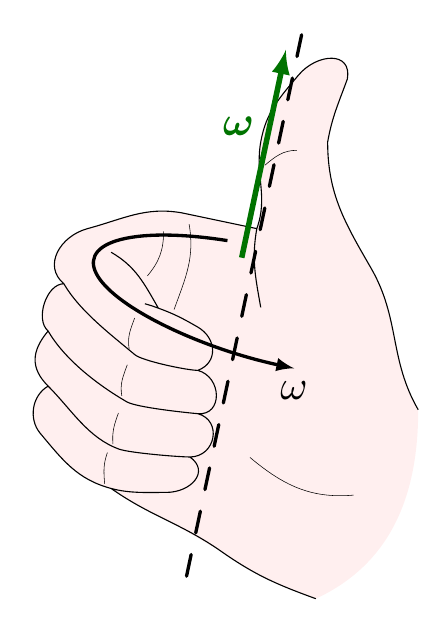
\begin{tikzpicture}
  \coordinate (O) at (1.1,0.2); % ORIGIN
  \coordinate (WT) at ( 2.9,-1.1); % WRIST TOP
  \coordinate (T1) at ( 2.3, 0.7); % THUMB
  \coordinate (T2) at ( 1.75, 2.3);
  \coordinate (T3) at ( 2.0, 3.1);
  \coordinate (T4) at (1.38, 3.15);
  \coordinate (T5) at ( 0.9, 2.3);
  \coordinate (T6) at ( 0.85, 1.2);
  \coordinate (T7) at ( 0.9, 0.2);
  \coordinate (I1) at (-0.1, 1.4); % INDEX
  \coordinate (I2) at (-1.3, 1.2);
  \coordinate (I3) at (-1.6, 0.5);
  \coordinate (I4) at (-0.7,-0.4);
  \coordinate (I5) at ( 0.1,-0.6);
  \coordinate (I6) at ( 0.1,-0.05);
  \coordinate (I7) at (-0.4,0.19);
  \coordinate (I8) at (-1.0, 0.9);
  \coordinate (M1) at (-1.8,-0.1); % MIDDLE
  %\coordinate (M2) at (-0.5,-0.7);
  \coordinate (M2) at (-0.8,-1.0);
  \coordinate (M3) at ( 0.1,-1.15);
  \coordinate (R1) at (-1.8,-0.8); % RING
  \coordinate (R2) at (-0.9,-1.6);
  \coordinate (R3) at (-0.0,-1.7);
  \coordinate (R4) at ( 0.0,-1.1);
  \coordinate (P1) at (-1.9,-1.4); % PINKY
  \coordinate (P2) at (-1.0,-2.1);
  \coordinate (P3) at (-0.3,-2.15);
  \coordinate (W1) at ( 0.4,-2.9); % WRIST BOTTOM
  \coordinate (W2) at ( 1.6,-3.5);
  
  % HAND
  \fill[pinkskin]
    (WT) -- (T6) -- (I2) -- (P2) -- (W1) -- (W2) to[out=25,in=-90] cycle;
  \draw[fill=pinkskin]
    (WT) to[out=120,in=-60] % THUMB
    (T1) to[out=120,in=-90]
    (T2) to[out=80,in=-110]
    (T3) to[out=80,in=50,looseness=1.5] % tip
    (T4) to[out=-130,in=80]
    (T5) to[out=-100,in=70]
    (T6) to[out=-100,in=100]
    (T7)
    (T6) -- % INDEX
    (I1) to[out=170,in=15]
    (I2) to[out=-165,in=140,looseness=1.2] % knuckle
    (I3) to[out=-60,in=140,looseness=0.8]
    (I4) to[out=-40,in=180,looseness=0.4]
    (I5) to[out=20,in=-30,looseness=1.3] % tip
    (I6) to[out=150,in=-20]
    (I7) to[out=120,in=-30]
    (I8)
    (I7) to[out=160,in=-15]++ (162:0.18)
    (I3) to[out=180,in=140,looseness=0.9] % MIDDLE
    (M1) to[out=-60,in=150,looseness=0.8]
    (M2) to[out=-30,in=175,looseness=0.4]
    (M3) to[out=-5,in=-15,looseness=1.5] % tip
    (I5)
    (M1) to[out=-130,in=135,looseness=1.2] % knuckle
    (R1) to[out=-45,in=160,looseness=0.9]
    (R2) to[out=-20,in=180,looseness=0.4]
    (R3) to[out=0,in=-15,looseness=1.5] % tip
    (M3)
    (R1) to[out=-150,in=130] % PINKY
    (P1) to[out=-50,in=165]
    (P2) to[out=-15,in=180,looseness=0.9]
    (P3) to[out=0,in=-35,looseness=1.5] % tip
    (R3)
    (P2) to[out=-35,in=145] % WRIST
    (W1) to[out=-35,in=160]
    (W2);
  
  % FOLDS
  \draw[very thin] (T5)++(-80:0.3) to[out=40,in=180]++ (25:0.45); % THUMB
  \draw[very thin] (I4)++(135:0.1) to[out=100,in=-110]++ (80:0.4); % INDEX
  \draw[very thin] (M2)++(130:0.1) to[out=100,in=-110]++ (80:0.4); % MIDDLE
  \draw[very thin] (R2)++(140:0.1) to[out=95,in=-110]++ (80:0.4); % RING
  \draw[very thin] (P2)++(145:0.1) to[out=95,in=-110]++ (85:0.4); % PINKY
  \draw[very thin] (I8)++(-33:0.55) to[out=50,in=-90]++ (70:0.6); % PALM
  \draw[very thin] (I7)++(-5:0.2) to[out=70,in=-80]++ (80:1.1); % PALM
  \draw[very thin] (W2)++(70:1.4) to[out=-175,in=-40]++ (160:1.4); % PALM
  
  % VECTORS
  \def\Rx{2.4}
  \def\Ry{0.7}
  \draw[very thick,dash pattern=on 8pt off 8pt,line cap=round]
    (O)++(-108.5:3.6) --++ (78:7.1);
  \draw[vector]
    (O)++(125:0.77) --++ (78:2.7)
    node[midway,above=10,left=-3,scale=1.5] {$\vb*{\omega}$};
  \draw[->,very thick,rotate=-15]
    (O)++(-250:{\Rx} and {\Ry}) arc (-250:-80:{\Rx} and {\Ry})
    node[below=-1,scale=1.5] {$\omega$};
  
\end{tikzpicture}


% RIGHT HAND RULE - angular momentum
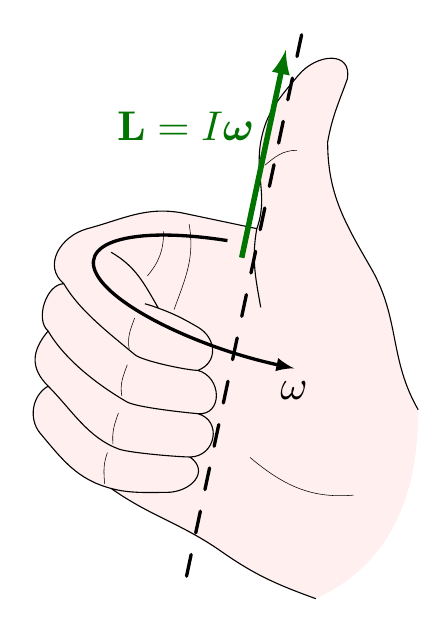
\begin{tikzpicture}
  \coordinate (O) at (1.1,0.2); % ORIGIN
  \coordinate (WT) at ( 2.9,-1.1); % WRIST TOP
  \coordinate (T1) at ( 2.3, 0.7); % THUMB
  \coordinate (T2) at ( 1.75, 2.3);
  \coordinate (T3) at ( 2.0, 3.1);
  \coordinate (T4) at (1.38, 3.15);
  \coordinate (T5) at ( 0.9, 2.3);
  \coordinate (T6) at ( 0.85, 1.2);
  \coordinate (T7) at ( 0.9, 0.2);
  \coordinate (I1) at (-0.1, 1.4); % INDEX
  \coordinate (I2) at (-1.3, 1.2);
  \coordinate (I3) at (-1.6, 0.5);
  \coordinate (I4) at (-0.7,-0.4);
  \coordinate (I5) at ( 0.1,-0.6);
  \coordinate (I6) at ( 0.1,-0.05);
  \coordinate (I7) at (-0.4,0.19);
  \coordinate (I8) at (-1.0, 0.9);
  \coordinate (M1) at (-1.8,-0.1); % MIDDLE
  %\coordinate (M2) at (-0.5,-0.7);
  \coordinate (M2) at (-0.8,-1.0);
  \coordinate (M3) at ( 0.1,-1.15);
  \coordinate (R1) at (-1.8,-0.8); % RING
  \coordinate (R2) at (-0.9,-1.6);
  \coordinate (R3) at (-0.0,-1.7);
  \coordinate (R4) at ( 0.0,-1.1);
  \coordinate (P1) at (-1.9,-1.4); % PINKY
  \coordinate (P2) at (-1.0,-2.1);
  \coordinate (P3) at (-0.3,-2.15);
  \coordinate (W1) at ( 0.4,-2.9); % WRIST BOTTOM
  \coordinate (W2) at ( 1.6,-3.5);
  
  % HAND
  \fill[pinkskin]
    (WT) -- (T6) -- (I2) -- (P2) -- (W1) -- (W2) to[out=25,in=-90] cycle;
  \draw[fill=pinkskin]
    (WT) to[out=120,in=-60] % THUMB
    (T1) to[out=120,in=-90]
    (T2) to[out=80,in=-110]
    (T3) to[out=80,in=50,looseness=1.5] % tip
    (T4) to[out=-130,in=80]
    (T5) to[out=-100,in=70]
    (T6) to[out=-100,in=100]
    (T7)
    (T6) -- % INDEX
    (I1) to[out=170,in=15]
    (I2) to[out=-165,in=140,looseness=1.2] % knuckle
    (I3) to[out=-60,in=140,looseness=0.8]
    (I4) to[out=-40,in=180,looseness=0.4]
    (I5) to[out=20,in=-30,looseness=1.3] % tip
    (I6) to[out=150,in=-20]
    (I7) to[out=120,in=-30]
    (I8)
    (I7) to[out=160,in=-15]++ (162:0.18)
    (I3) to[out=180,in=140,looseness=0.9] % MIDDLE
    (M1) to[out=-60,in=150,looseness=0.8]
    (M2) to[out=-30,in=175,looseness=0.4]
    (M3) to[out=-5,in=-15,looseness=1.5] % tip
    (I5)
    (M1) to[out=-130,in=135,looseness=1.2] % knuckle
    (R1) to[out=-45,in=160,looseness=0.9]
    (R2) to[out=-20,in=180,looseness=0.4]
    (R3) to[out=0,in=-15,looseness=1.5] % tip
    (M3)
    (R1) to[out=-150,in=130] % PINKY
    (P1) to[out=-50,in=165]
    (P2) to[out=-15,in=180,looseness=0.9]
    (P3) to[out=0,in=-35,looseness=1.5] % tip
    (R3)
    (P2) to[out=-35,in=145] % WRIST
    (W1) to[out=-35,in=160]
    (W2);
  
  % FOLDS
  \draw[very thin] (T5)++(-80:0.3) to[out=40,in=180]++ (25:0.45); % THUMB
  \draw[very thin] (I4)++(135:0.1) to[out=100,in=-110]++ (80:0.4); % INDEX
  \draw[very thin] (M2)++(130:0.1) to[out=100,in=-110]++ (80:0.4); % MIDDLE
  \draw[very thin] (R2)++(140:0.1) to[out=95,in=-110]++ (80:0.4); % RING
  \draw[very thin] (P2)++(145:0.1) to[out=95,in=-110]++ (85:0.4); % PINKY
  \draw[very thin] (I8)++(-33:0.55) to[out=50,in=-90]++ (70:0.6); % PALM
  \draw[very thin] (I7)++(-5:0.2) to[out=70,in=-80]++ (80:1.1); % PALM
  \draw[very thin] (W2)++(70:1.4) to[out=-175,in=-40]++ (160:1.4); % PALM
  
  % VECTORS
  \def\Rx{2.4}
  \def\Ry{0.7}
  \draw[very thick,dash pattern=on 8pt off 8pt,line cap=round]
    (O)++(-108.5:3.6) --++ (78:7.1);
  \draw[vector]
    (O)++(125:0.77) --++ (78:2.7)
    node[midway,above=10,left=-3,scale=1.5] {$\vb{L} = I\vb*{\omega}$};
  \draw[->,very thick,rotate=-15]
    (O)++(-250:{\Rx} and {\Ry}) arc (-250:-80:{\Rx} and {\Ry})
    node[below=-1,scale=1.5] {$\omega$};
  
\end{tikzpicture}


% RIGHT HAND RULE - magnetic moment
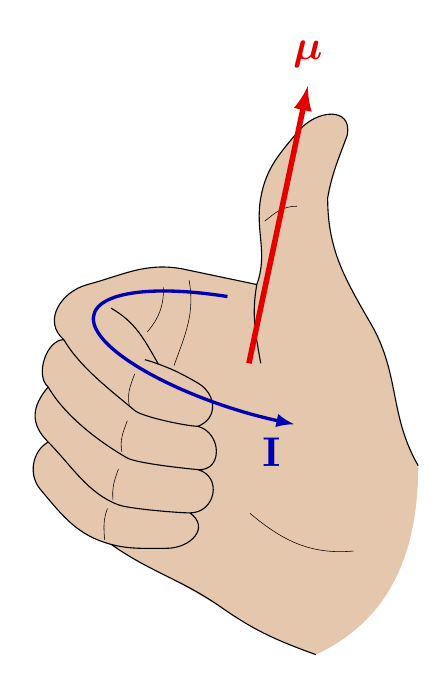
\begin{tikzpicture}
  \coordinate (O) at (1.1,0.2); % ORIGIN
  \coordinate (WT) at ( 2.9,-1.1); % WRIST TOP
  \coordinate (T1) at ( 2.3, 0.7); % THUMB
  \coordinate (T2) at ( 1.75, 2.3);
  \coordinate (T3) at ( 2.0, 3.1);
  \coordinate (T4) at (1.38, 3.15);
  \coordinate (T5) at ( 0.9, 2.3);
  \coordinate (T6) at ( 0.85, 1.2);
  \coordinate (T7) at ( 0.9, 0.2);
  \coordinate (I1) at (-0.1, 1.4); % INDEX
  \coordinate (I2) at (-1.3, 1.2);
  \coordinate (I3) at (-1.6, 0.5);
  \coordinate (I4) at (-0.7,-0.4);
  \coordinate (I5) at ( 0.1,-0.6);
  \coordinate (I6) at ( 0.1,-0.05);
  \coordinate (I7) at (-0.4,0.19);
  \coordinate (I8) at (-1.0, 0.9);
  \coordinate (M1) at (-1.8,-0.1); % MIDDLE
  %\coordinate (M2) at (-0.5,-0.7);
  \coordinate (M2) at (-0.8,-1.0);
  \coordinate (M3) at ( 0.1,-1.15);
  \coordinate (R1) at (-1.8,-0.8); % RING
  \coordinate (R2) at (-0.9,-1.6);
  \coordinate (R3) at (-0.0,-1.7);
  \coordinate (R4) at ( 0.0,-1.1);
  \coordinate (P1) at (-1.9,-1.4); % PINKY
  \coordinate (P2) at (-1.0,-2.1);
  \coordinate (P3) at (-0.3,-2.15);
  \coordinate (W1) at ( 0.4,-2.9); % WRIST BOTTOM
  \coordinate (W2) at ( 1.6,-3.5);
  
  % HAND
  \fill[brownskin]
    (WT) -- (T6) -- (I2) -- (P2) -- (W1) -- (W2) to[out=25,in=-90] cycle;
  \draw[fill=brownskin]
    (WT) to[out=120,in=-60] % THUMB
    (T1) to[out=120,in=-90]
    (T2) to[out=80,in=-110]
    (T3) to[out=80,in=50,looseness=1.5] % tip
    (T4) to[out=-130,in=80]
    (T5) to[out=-100,in=70]
    (T6) to[out=-100,in=100]
    (T7)
    (T6) -- % INDEX
    (I1) to[out=170,in=15]
    (I2) to[out=-165,in=140,looseness=1.2] % knuckle
    (I3) to[out=-60,in=140,looseness=0.8]
    (I4) to[out=-40,in=180,looseness=0.4]
    (I5) to[out=20,in=-30,looseness=1.3] % tip
    (I6) to[out=150,in=-20]
    (I7) to[out=120,in=-30]
    (I8)
    (I7) to[out=160,in=-15]++ (162:0.18)
    (I3) to[out=180,in=140,looseness=0.9] % MIDDLE
    (M1) to[out=-60,in=150,looseness=0.8]
    (M2) to[out=-30,in=175,looseness=0.4]
    (M3) to[out=-5,in=-15,looseness=1.5] % tip
    (I5)
    (M1) to[out=-130,in=135,looseness=1.2] % knuckle
    (R1) to[out=-45,in=160,looseness=0.9]
    (R2) to[out=-20,in=180,looseness=0.4]
    (R3) to[out=0,in=-15,looseness=1.5] % tip
    (M3)
    (R1) to[out=-150,in=130] % PINKY
    (P1) to[out=-50,in=165]
    (P2) to[out=-15,in=180,looseness=0.9]
    (P3) to[out=0,in=-35,looseness=1.5] % tip
    (R3)
    (P2) to[out=-35,in=145] % WRIST
    (W1) to[out=-35,in=160]
    (W2);
  
  % FOLDS
  \draw[very thin] (T5)++(-80:0.3) to[out=40,in=180]++ (25:0.45); % THUMB
  \draw[very thin] (I4)++(135:0.1) to[out=100,in=-110]++ (80:0.4); % INDEX
  \draw[very thin] (M2)++(130:0.1) to[out=100,in=-110]++ (80:0.4); % MIDDLE
  \draw[very thin] (R2)++(140:0.1) to[out=95,in=-110]++ (80:0.4); % RING
  \draw[very thin] (P2)++(145:0.1) to[out=95,in=-110]++ (85:0.4); % PINKY
  \draw[very thin] (I8)++(-33:0.55) to[out=50,in=-90]++ (70:0.6); % PALM
  \draw[very thin] (I7)++(-5:0.2) to[out=70,in=-80]++ (80:1.1); % PALM
  \draw[very thin] (W2)++(70:1.4) to[out=-175,in=-40]++ (160:1.4); % PALM
  
  % VECTORS
  \def\Rx{2.4}
  \def\Ry{0.7}
  \draw[mu vector]
    (O)++(-180:0.35) --++ (78:3.6)
    node[above,scale=1.5] {$\vb*{\mu}$};
  %\draw[thick,rotate=-15]
  %  (O) ellipse ({\Rx} and {\Ry}); %++({\Rx*(1-cos(250))},{-\Ry*sin(250))})
  \draw[current,very thick,rotate=-15]
    (O)++(-250:{\Rx} and {\Ry}) arc (-250:-80:{\Rx} and {\Ry})
    node[below left=-1,scale=1.5] {$\vb{I}$};
    
%  % HELP LINES
%  \foreach \i in {0,...,4}{
%    \draw[very thin,red!10] (-4.5, \i) -- (4, \i) node[red!30] {\i};
%    \draw[very thin,red!10] (-4.5,-\i) -- (4,-\i) node[red!30] {-\i};
%    \draw[very thin,red!10] (\i,-4) -- (\i,4) node[red!30] {\i};
%    \draw[very thin,red!10] (-\i,-4) -- (-\i,4) node[red!30] {-\i};
%  }
%  \node[blue,scale=0.4] at (T1) {T1};
%  \node[blue,scale=0.4] at (T2) {T2};
%  \node[blue,scale=0.4] at (T3) {T3};
%  \node[blue,scale=0.4] at (T4) {T4};
%  \node[blue,scale=0.4] at (T5) {T5};
%  \node[blue,scale=0.4] at (T6) {T6};
%  \node[blue,scale=0.4] at (T7) {T7};
%  \node[blue,scale=0.4] at (I1) {I1};
%  \node[blue,scale=0.4] at (I2) {I2};
%  \node[blue,scale=0.4] at (I3) {I3};
%  \node[blue,scale=0.4] at (I4) {I4};
%  \node[blue,scale=0.4] at (I5) {I5};
%  \node[blue,scale=0.4] at (I6) {I6};
%  \node[blue,scale=0.4] at (I7) {I7};
%  \node[blue,scale=0.4] at (I8) {I8};
%  \node[blue,scale=0.4] at (M1) {M1};
%  \node[blue,scale=0.4] at (M2) {M2};
%  \node[blue,scale=0.4] at (M3) {M3};
%  \node[blue,scale=0.4] at (R1) {R1};
%  \node[blue,scale=0.4] at (R2) {R2};
%  \node[blue,scale=0.4] at (R3) {R3};
%  \node[blue,scale=0.4] at (P1) {P1};
%  \node[blue,scale=0.4] at (P2) {P2};
%  \node[blue,scale=0.4] at (P3) {P3};
%  %\node[blue,scale=0.4] at (P4) {P4};
%  \node[blue,scale=0.4] at (W1) {W1};
%  \node[blue,scale=0.4] at (W2) {W2};
  
\end{tikzpicture}



% RIGHT HAND RULE - magnetic moment
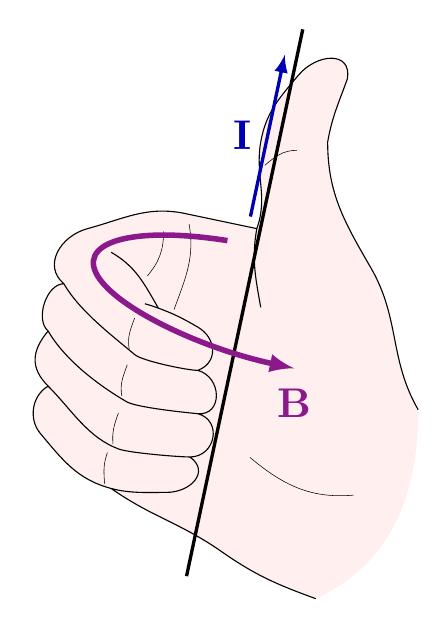
\begin{tikzpicture}
  \coordinate (O) at (1.1,0.2); % ORIGIN
  \coordinate (WT) at ( 2.9,-1.1); % WRIST TOP
  \coordinate (T1) at ( 2.3, 0.7); % THUMB
  \coordinate (T2) at ( 1.75, 2.3);
  \coordinate (T3) at ( 2.0, 3.1);
  \coordinate (T4) at (1.38, 3.15);
  \coordinate (T5) at ( 0.9, 2.3);
  \coordinate (T6) at ( 0.85, 1.2);
  \coordinate (T7) at ( 0.9, 0.2);
  \coordinate (I1) at (-0.1, 1.4); % INDEX
  \coordinate (I2) at (-1.3, 1.2);
  \coordinate (I3) at (-1.6, 0.5);
  \coordinate (I4) at (-0.7,-0.4);
  \coordinate (I5) at ( 0.1,-0.6);
  \coordinate (I6) at ( 0.1,-0.05);
  \coordinate (I7) at (-0.4,0.19);
  \coordinate (I8) at (-1.0, 0.9);
  \coordinate (M1) at (-1.8,-0.1); % MIDDLE
  %\coordinate (M2) at (-0.5,-0.7);
  \coordinate (M2) at (-0.8,-1.0);
  \coordinate (M3) at ( 0.1,-1.15);
  \coordinate (R1) at (-1.8,-0.8); % RING
  \coordinate (R2) at (-0.9,-1.6);
  \coordinate (R3) at (-0.0,-1.7);
  \coordinate (R4) at ( 0.0,-1.1);
  \coordinate (P1) at (-1.9,-1.4); % PINKY
  \coordinate (P2) at (-1.0,-2.1);
  \coordinate (P3) at (-0.3,-2.15);
  \coordinate (W1) at ( 0.4,-2.9); % WRIST BOTTOM
  \coordinate (W2) at ( 1.6,-3.5);
  
  % HAND
  \fill[pinkskin]
    (WT) -- (T6) -- (I2) -- (P2) -- (W1) -- (W2) to[out=25,in=-90] cycle;
  \draw[fill=pinkskin]
    (WT) to[out=120,in=-60] % THUMB
    (T1) to[out=120,in=-90]
    (T2) to[out=80,in=-110]
    (T3) to[out=80,in=50,looseness=1.5] % tip
    (T4) to[out=-130,in=80]
    (T5) to[out=-100,in=70]
    (T6) to[out=-100,in=100]
    (T7)
    (T6) -- % INDEX
    (I1) to[out=170,in=15]
    (I2) to[out=-165,in=140,looseness=1.2] % knuckle
    (I3) to[out=-60,in=140,looseness=0.8]
    (I4) to[out=-40,in=180,looseness=0.4]
    (I5) to[out=20,in=-30,looseness=1.3] % tip
    (I6) to[out=150,in=-20]
    (I7) to[out=120,in=-30]
    (I8)
    (I7) to[out=160,in=-15]++ (162:0.18)
    (I3) to[out=180,in=140,looseness=0.9] % MIDDLE
    (M1) to[out=-60,in=150,looseness=0.8]
    (M2) to[out=-30,in=175,looseness=0.4]
    (M3) to[out=-5,in=-15,looseness=1.5] % tip
    (I5)
    (M1) to[out=-130,in=135,looseness=1.2] % knuckle
    (R1) to[out=-45,in=160,looseness=0.9]
    (R2) to[out=-20,in=180,looseness=0.4]
    (R3) to[out=0,in=-15,looseness=1.5] % tip
    (M3)
    (R1) to[out=-150,in=130] % PINKY
    (P1) to[out=-50,in=165]
    (P2) to[out=-15,in=180,looseness=0.9]
    (P3) to[out=0,in=-35,looseness=1.5] % tip
    (R3)
    (P2) to[out=-35,in=145] % WRIST
    (W1) to[out=-35,in=160]
    (W2);
  
  % FOLDS
  \draw[very thin] (T5)++(-80:0.3) to[out=40,in=180]++ (25:0.45); % THUMB
  \draw[very thin] (I4)++(135:0.1) to[out=100,in=-110]++ (80:0.4); % INDEX
  \draw[very thin] (M2)++(130:0.1) to[out=100,in=-110]++ (80:0.4); % MIDDLE
  \draw[very thin] (R2)++(140:0.1) to[out=95,in=-110]++ (80:0.4); % RING
  \draw[very thin] (P2)++(145:0.1) to[out=95,in=-110]++ (85:0.4); % PINKY
  \draw[very thin] (I8)++(-33:0.55) to[out=50,in=-90]++ (70:0.6); % PALM
  \draw[very thin] (I7)++(-5:0.2) to[out=70,in=-80]++ (80:1.1); % PALM
  \draw[very thin] (W2)++(70:1.4) to[out=-175,in=-40]++ (160:1.4); % PALM
  
  % VECTORS
  \def\Rx{2.4}
  \def\Ry{0.7}
  \draw[very thick]
    (O)++(-108.5:3.6) --++ (78:7.1);
  \draw[current,very thick]
    (O)++(106:1.2) --++ (78:2.1)
    node[midway,left,scale=1.5] {$\vb{I}$};
  \draw[BField,rotate=-15]
    (O)++(-250:{\Rx} and {\Ry}) arc (-250:-80:{\Rx} and {\Ry})
    node[below=1,scale=1.5] {$\vb{B}$};
  
\end{tikzpicture}


\end{document}